%!TEX program = xelatex
% this CV is modified from a template. Most of setting options and information can be found on https://www.overleaf.com/articles/odilia-almeidas-cv/yfqgvkrnjygs
\documentclass[11pt,a4paper,sans]{moderncv}
\moderncvstyle{banking}
\moderncvcolor{green}
% character encoding
\usepackage[utf8]{inputenc}
\usepackage{xeCJK}
\usepackage[left=2cm, right=2cm, top=1.7cm]{geometry}
\usepackage{import}
\usepackage{graphicx} 

% personal data
\name{Meng-Shr Tsai}{蔡孟師} 
\phone[mobile]{0968778062}
\email{qetup1988@gmail.com}
\homepage{collieiscute.github.io}
\begin{document}
\raisebox{-0.5\height}{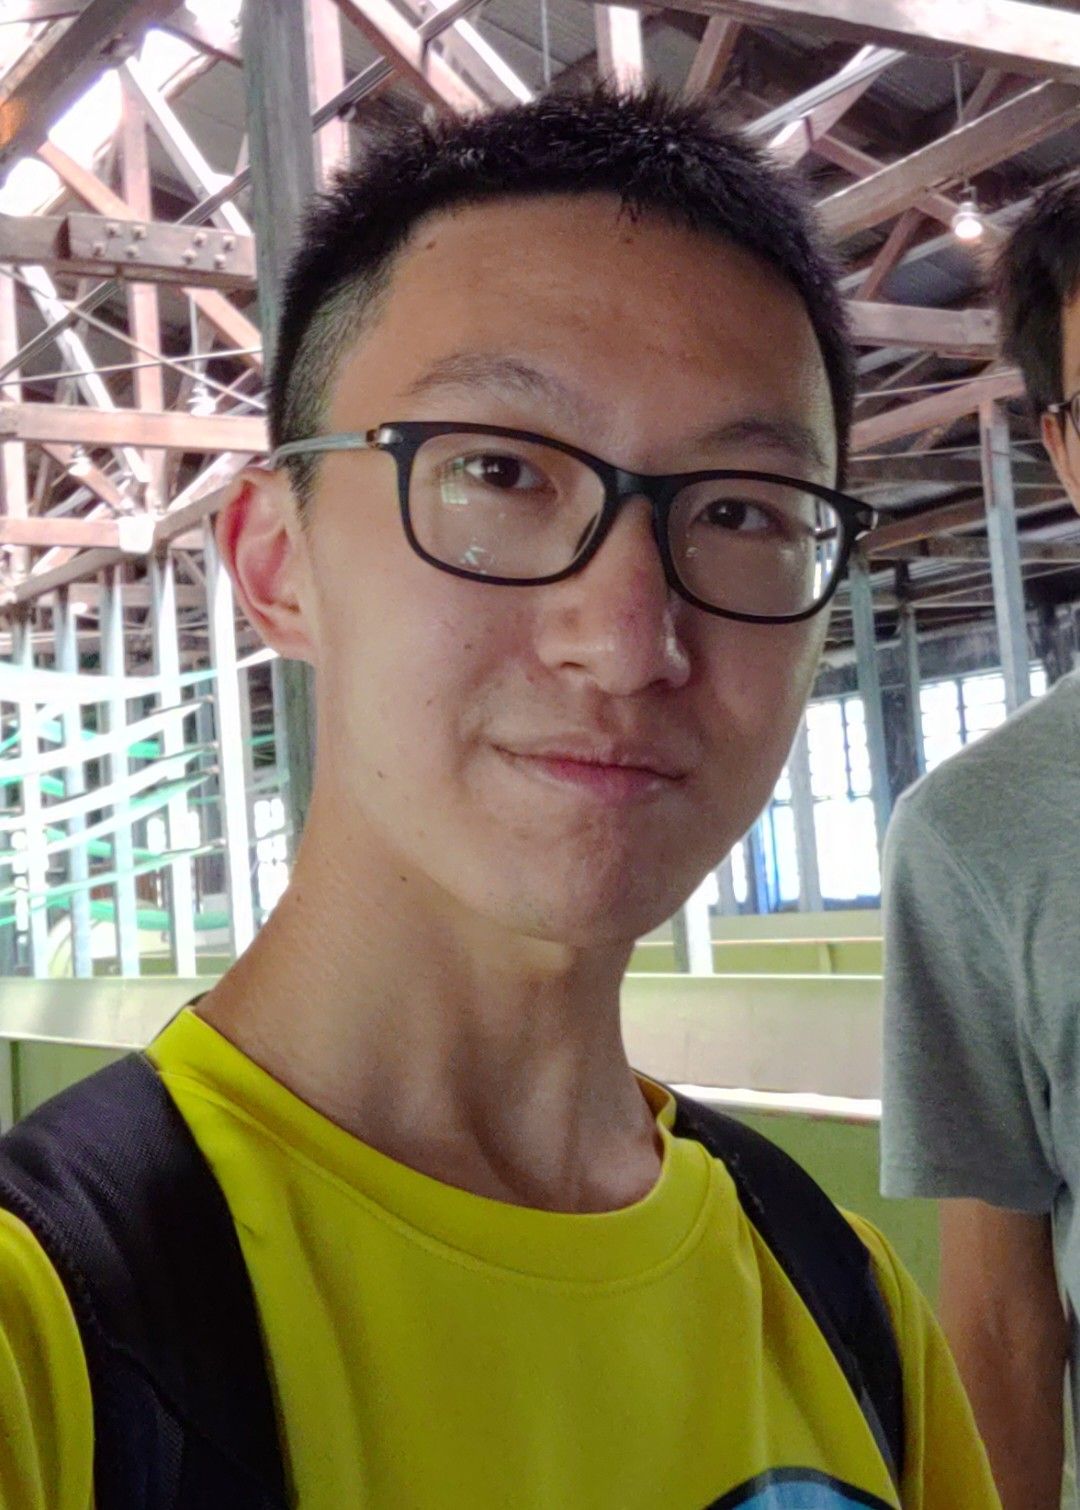
\includegraphics[width=3cm]{./images/head.jpg}}
\makecvtitle
\vspace{-20pt}
\section{Education}
\begin{itemize}
	\item{\cventry{Sep 2018 -- Jun 2022}{B.S. in computer science and engineering}{National Sun Yat-sen University (NSYSU)}{ Kaohsiung City, Taiwan}{}{}} \vspace{4pt}
\end{itemize}
	
\section{Skills}
\begin{itemize}
	\item Programming
	\begin{itemize}
		\item General: Modern C++(11 and a little 14~20), C, python3, Shell script
		\item Others: Arduino(C++11), Git, \LaTeX , Markdown
	\end{itemize}
	\item Languages
	\begin{itemize}
		\item native: Taiwan Mandarin, Taiwanese
		\item conversant: English (TOEIC 645)
	\end{itemize}
\end{itemize}
	
\section{Experience}

\vspace{4pt}

\begin{itemize}

\item{\cventry{Décembre 2014 -- Mars 2017}{Chef de Publicité}{Globosat - Chaîne GNT}{ Rio de Janeiro,Brésil}{}{\vspace{3pt} 
\begin{itemize}
\item Élaboration des campagnes et des stratégies de marketing pour les annonceurs.
\item Gestion des campagnes de marketing online et offline.
\item  Production des programmes et des vidéos personnalisés pour les marques des annonceurs sur support telévision et site web.
\item Préparation et coordination des projets de placement de produit et de merchandising pour les clients.
\end{itemize}
}}

\vspace{4pt}

\item{\cventry{Novembre 2011 -- Novembre 2014}{Assistante de Contenu}{Globosat - Chaîne GNT}{Rio de Janeiro, Brésil}{}{\vspace{3pt}
\begin{itemize}
\item  Gestion de la production et de la post-production des programmes et des séries télévisées.
\item  Intégration de tous les secteurs de la chaîne pour la diffusion du contenu.
\item  Production du contenu et de la mise en scène des saisons de la mode Fashion Rio et São Paulo Fashion Week.
\end{itemize}
}}

\vspace{4pt}

\item{\cventry{Novembre 2010 - Novembre 2011}{Stagiaire Production}{Globosat - Chaîne GNT}{Rio de Janeiro, Brésil}{}{\vspace{3pt}
\begin{itemize}
\item  Gestion de la production des programmes et des séries télévisées.
\item  Enregistrement de l'information concernant les programmes sur le site web de la chaîne.
\item  Production de contenu pour les réseaux sociaux de la chaîne.
\end{itemize}
}}

\vspace{4pt}

\item{\cventry{Novembre 2009 - Août 2010}{Stagiaire Communication Internationale}{Petrobras}{Rio de Janeiro, Brésil}{}{\vspace{3pt}
\begin{itemize}
\item  Soutien aux activités du département, incluant la production de la revue d'entreprise et des plaquettes institutionnelles.
\end{itemize}
}}
\end{itemize}

\section{Formation}

\vspace{4pt}

\begin{itemize}

\item{\cventry{2014 -- 2015}{ Rio de Janeiro}{Master en Marketing*}{PUC Université}{\textit{Brésil}}{}}

\item{\cventry{2007 -- 2011}{ Rio de Janeiro}{Maitrise en Communication Sociale - Journalisme*}{PUC Université}{\textit{Brésil}}{}}
* Attestation de comparabilité obtenue via le Département de reconnaissance des diplômes (CIEP)
\end{itemize}

\vspace{2pt}

\section{Langues}

\vspace{1pt}

\begin{itemize}

\item \textbf{Anglais:} Courant, Capacité Professionelle Complète 

\vspace{1pt}

\item \textbf{Français:} Courant, Capacité Professionelle Complète 

\vspace{1pt}

\item \textbf{Espagnol:} Courant, Compétence Professionnelle

\vspace{1pt}

\item \textbf{Portugais:} Langue maternelle

\end{itemize}
\end{document}


%% end of file `template.tex'.